% -*- TeX-master: "main"; fill-column: 72 -*-

\section{Examples}
\label{examples}

This section contains a variety of examples of SBML Level~3 Version~1
documents employing the Flux Balance Constraints package.

\subsection{\FBC syntax examples}

These examples are provided to highlight the \FBCPackage syntax.

\subsubsection{Example One}

\begin{figure}[h]
  \centering
  % Requires \usepackage{graphicx}
  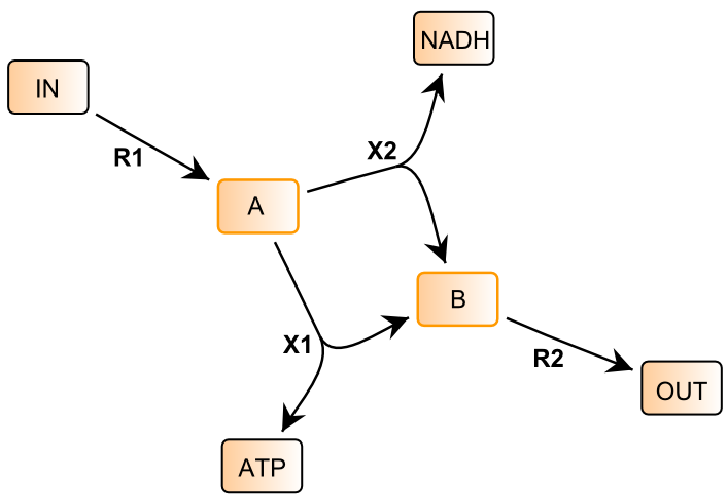
\includegraphics[width=8cm]{examples/spec-example1.pdf}\\
  \caption{\FBC syntax example: a simple four reaction pathway. The
  reactions are \textit{R1}, \textit{R2}, \textit{X1}, \textit{X2} with
  fixed species \textit{IN}, \textit{OUT}, \textit{ATP}, \textit{NADH} and
  variable species \textit{A}, \textit{B}.}
  \label{fig:example1}
\end{figure}

As shown in \ref{fig:example1} the first example is a simple four reaction
pathway that transforms metabolite \textit{IN} to \textit{OUT}. To begin
with it is possible to compactly describe this network in terms of its
reaction stoichiometry as shown in \ref{tble:ex1nmat}.
\begin{table}[h]
  \centering
    \begin{tabular}{c|cccc}
          & R1 & R2 & X1 & X2 \\ \hline
        A & 1 &  0 & -1 & -1 \\
        B & 0 & -1 &  1 &  1 \\
    \end{tabular}
  \caption{Example one: stoichiometric matrix, \Nmat}
  \label{tble:ex1nmat}
\end{table}
%
While the stoichiometry contains the structural properties of the reaction
network the full description of a biological model can be described as a set
of ordinary differential equations (ODE's). While other formalisms may exist
here we will concentrate exclusively on kinetic models where the change in
concentration of each variable component in the system ($\frac{ds}{dt}$) is
a non-linear function of the rates of the reactions which either create or
consume it (the product of the stoichiometric matrix, \Nmat\ and the vector
of reaction rates, \vvec).
%
\begin{equation}\label{eqn:kinmod}
  \frac{ds}{dt} = \textbf{Nv}
\end{equation}
%
The formulation of the kinetic model, as shown in Equation~\ref{eqn:kinmod}
is typical of the kind that can already be described using `traditional'
\SBML where the vector \vvec\ would contain rate equations as a function of
parameters and concentrations. In the XML representation of this model
provided below the reaction stoichiometry is captured in the \Species and
\Reaction definitions. In a constraint based model these rate laws are
considered unknowns and the system is assumed to be in steady state (see
Equation~\ref{eqn:kinmodsteady}):
%
\begin{equation}\label{eqn:kinmodsteady}
  \textbf{NJ} = 0
\end{equation}
%
Note how the rate vector \vvec\ is now represented as the flux vector \Jvec.
To perform a typical steady-state analysis such as flux balance analysis
(FBA) we need to include to more pieces of information into our model
description:
%
\begin{enumerate}
  \item A capacity constraint: the maximum limit (upper bound) of the flux
      through reaction \textit{R1} is 1 (with an arbitrary unit of flux).
  \item An objective target which can be maximized or minimized: in this
      example the  flux through reaction \textit{R2} will be
      \textit{maximized}.
\end{enumerate}
%
However, \sbmlthreecore does not have an unambiguous way of encoding either
a capacity constraint or an objective target and for this we now need to use
the additional constructs provided by the \FBCPackage. In the example XML
shown below, this additional information is encoded from Line~83--92.
Encoded in this way the constraint based model can now be formulated as a
Linear Program and analyzed using FBA (here shown in LP format as used by
IBM CPLEX):
%
\exampleFile{examples/spec-example1.lp}
%
Solving this problem we find that maximization of flux through \textit{R2}
gives an optimal solution of \textit{one} shown with one possible solution
for \Jvec\ (see Equation~\ref{egn:ex1sol1}).
\begin{equation}\label{egn:ex1sol1}
  \left(
    \begin{array}{cccc}
        1 &  0 & -1 & -1 \\
        0 & -1 &  1 &  1 \\
    \end{array}
  \right)
  \left(
    \begin{array}{c}
        1.0 \\
        1.0 \\
        0.0 \\
        1.0 \\
    \end{array}
  \right)
  = \textbf{0}
\end{equation}

The following code block is the XML that represents the model described as
Example~One in the preceding text.
%
\exampleFile{examples/spec-example1.txt}
